\section{ステップ6:Dartエディタのリファクタリングツールを使用してコードをきれいにします}

リファクタリングは、コードの動作を変更せずにコードの構造を変化させる技術です。あなたがシステムを進化させるためには、コードをきれいにすることが重要です。最近の開発環境では、リファクタリングが自動化されていることでコードの保守を簡単にできます。

一般的なリファクタリングは、メソッド名、変数名、クラス名などを分かりやすくすることです。名前をわかりやすく維持することは、コードの健康のために重要です。Dartエディタでは名前変更のリファクタリングを自動で行うことができます。

\subsection{オブジェクティブ}

\begin{enumerate}
\item 自動的にメソッド名や変数名を変更する
\end{enumerate}

\subsection{コード}

コードラボのここから開始したい場合、step06をコピーして下さい。

\subsection{チュートリアル}

cliend/chat-client.dart ファイルを開き、一番上にスクロールしてください。自動的に変数名を変更するために、Dartエディタを使用します。

\subsubsection{変数名の変更}

ファイルの上の方にある ChatConnection connection オブジェクトを探します。connectionはパッと見で、何の接続を表しているのかが分かりにくいので、この変数名をもっとわかりやすく変更します。
(もちろん、ツールはWebSocketの接続であることを教えてくれますが、読みやすいコードの方が良いです)

connectionを右クリックして、[Rename]を選択します。

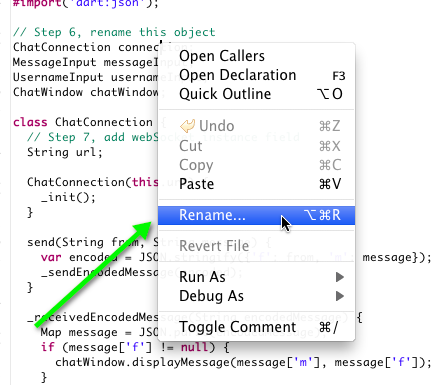
\includegraphics{step6/step6_img1.png}

変数名 connection がハイライトされ、新しい名前を入力できるようになります。より分かりやすくなるように chatConnection と入力して、Enterキーを押します。

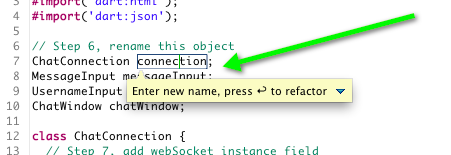
\includegraphics{step6/step6_img2.png}

\subsubsection{変更のレビュー}

ファイル全体の connection という名前が、 chatConnection に変更されました。ファイルの一番下まで確認してみて下さい。main()関数の内側が変更されたことが分かると思います。そして、MessageInputのbind() メソッドの内側の名前も変更されています。

また、Dartエディタの検索を使用してchatConnectionを検索することができます。

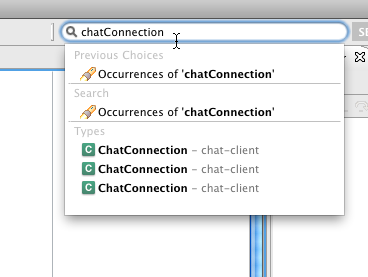
\includegraphics{step6/step6_img3.png}

\subsection{上級編}

他のメソッドや変数の名前を変更してみましょう。静的な型付けをされている変数や、varを利用した動的な型付けをされている変数でも試してみてください。

ヒント:上級編であまりにも多くの名前を変更した場合、今後のステップで少し混乱するかもしれないので、上級編で行った変更を元に戻すことをお勧めします。
